\documentclass{article}
%packages
\usepackage{graphicx}
\usepackage{minted}
\usepackage[utf8]{inputenc}
\usepackage[T1]{fontenc}
\usepackage[frenchb]{babel}
\usepackage[a4paper]{geometry}
\usepackage{hyperref}

\begin{document}
	%title
	\begin{titlepage}
		\vspace{-20px}
		\begin{tabular}{l}
			\textsc{Blin} Sébastien
		\end{tabular}
		\hfill \vspace{10px}
\includegraphics[scale=0.1]{esir}\\
		\vfill
		\begin{center}
			\Huge{\'Ecole sup\'erieure d'ing\'enieurs de Rennes}\\
			\vspace{1cm}
			\LARGE{2ème année}\\
			\large{Parcours Informatique}\\
			\vspace{0.5cm}\hrule\vspace{0.5cm}
			\LARGE{\textbf{TP 5-6 SPP}}\\
			\Large{Eratosthenes' Sieve}
			\vspace{0.5cm}\hrule
			\vfill
			\vfill
		\end{center}
		\begin{flushleft}
			\Large{Sous l'encadrement de~:}\\
			\vspace{0.2cm}
			\large{{Taïani} François}
		\end{flushleft}
		\vfill
	\end{titlepage}

\section{Task 1}
\label{sec:Task 1}

\begin{itemize}
	\item La première boucle ne va que jusqu'à $\sqrt{n}$ car on n'enleve que à partir de $i^2$. Or, $\sqrt{n}^2=n$ ce qui est notre limite maximale.
	\item La boucle interne commence à $i^2$ car 0 n'est pas dans le tableau et i peut etre un nombre premier. Donc \emph{A[0]} et \emph{A[i]} ne sont pas intéressant pour cette boucle
\end{itemize}

\section{Task 4}
\label{sec:Task 4}

\begin{itemize}
	\item Non, un moniteur ou un lock n'est pas nécessaire, car tous les threads souhaitent écrire la même chose. En effet, ils écrivent tous \emph{false} dans des cases.
\end{itemize}

\section{Task 5}
\label{sec:Task 5}

Voici le graph du benchmarking~:
\begin{center}
	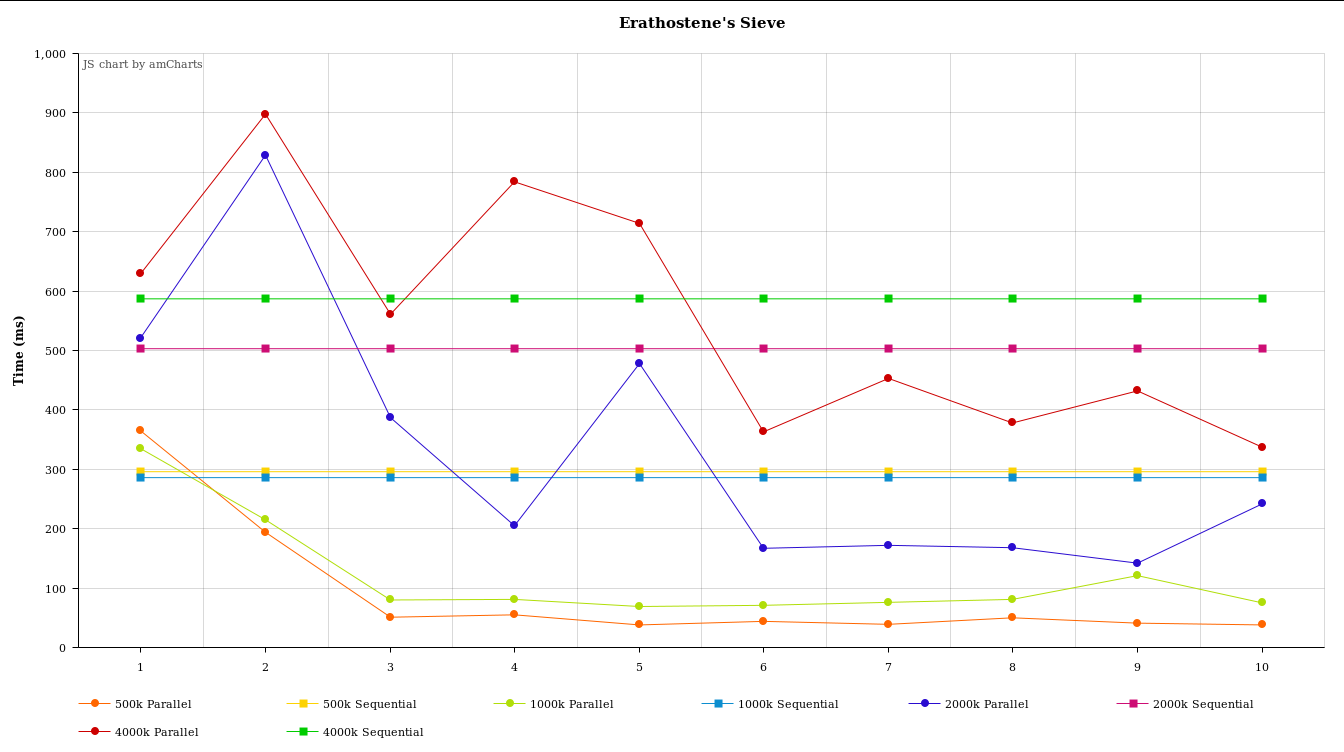
\includegraphics[scale=0.37]{../results/graphTests}\\
	Benchmarking
	\label{1}
\end{center}
\end{document}
